% ============================================================
% GSPH-FC (v3) — Springer LNCS
% Compilar: pdflatex -> bibtex -> pdflatex -> pdflatex
% Figuras: Resultados_v2/ (tours) y Resultados_v3/ (convergencia)
% Cómo regenerar cada tabla y figura: REPRODUCIR.md
% ============================================================
\documentclass[runningheads]{llncs}
\usepackage[T1]{fontenc}
\usepackage[utf8]{inputenc}
\usepackage{graphicx}
\usepackage{amsmath,amssymb}
\usepackage{booktabs}
\usepackage{algorithm}
\usepackage[noend]{algpseudocode}
\usepackage{url}

\begin{document}

\title{GSPH-FC: Geometric Partitioning with Frontier Connectivity
and a Localized Iterated Local Search for the Euclidean TSP}
\titlerunning{GSPH-FC for the Euclidean TSP}

\author{%
    Martín Gómez Navarro\inst{1} \and
    Rodrigo Linfati\inst{2} \and
    Juan Carlos Figueroa-García\inst{3} \and
    Carlos Alberto Franco Franco\inst{3} \and
    Daniel Morillo-Torres\inst{4} \and
    Jairo R. Coronado-Hernandez\inst{5} \and
    Gustavo Esteban Gatica\inst{1}}
\authorrunning{M. Gómez Navarro et al.}
\institute{%
    Faculty of Engineering, Universidad Andres Bello, Santiago, Chile\\
    \email{m.gmeznavarro@uandresbello.edu}\\
    \email{ggatica@uandresbello.edu}
    \and
    Faculty of Engineering, Universidad del Bío-Bío,
    Concepción, Chile\\
    \email{rlinfati@ubiobio.cl}
    \and
    Faculty of Engineering, Universidad Distrital
    Francisco José de Caldas, Bogotá, Colombia\\
    \email{jcfigueroag@udistrital.edu.co}
    \email{cafrancof@udistrital.edu.co}
    \and
    Faculty of Engineering, Pontificia Universidad Javeriana de Cali,
    Cali, Colombia\\
    \email{daniel.morillo@javerianacali.edu.co}
    \and
    Faculty of Engineering, Universidad de la Costa,
    Barranquilla, Colombia\\
    \email{jcoronad18@cuc.edu.co}}

\maketitle

\begin{abstract}
We present \textbf{GSPH-FC}, a heuristic for the Euclidean Traveling
Salesman Problem (TSP) with two parts. The first is a geometric
construction: the plane is split into four quadrants, the connections
between adjacent quadrants (frontier pairs) are chosen \emph{before} any
local route exists, and each quadrant is then routed as an open path
anchored at those connections. The second is a localized iterated local
search (ILS): neighbor-list 2-opt and Or-opt, a double-bridge confined
to a window that grows with the instance size, Metropolis acceptance,
undo through a log of segment reversals, and termination by stagnation,
all compiled to native code. On 77 TSPLIB instances with up to
18{,}512 cities, GSPH-FC reaches the best known solution (BKS) on 44,
including all 36 instances with $n\le 300$ in under 0.5~s each, and its
best tour stays within 0.60\% of the BKS up to 6{,}000 cities. Beyond
the benchmark, we measure where this quality comes from. An ablation
with the search engine held fixed shows that frontier connectivity gives
the best starting tours (9.95\% above the BKS against 24.71\% for
nearest neighbor) and the most BKS hits, while the localized ILS
accounts for most of the final quality. Convergence curves over time
show no early advantage of the full
construction, which pays an up-front cost: the ILS erases most of the
differences between starting tours within the first tenth of the run,
and geometric starts mainly help to avoid poor basins, such as those
nearest neighbor falls into on clustered instances.
A sensitivity study on 16 instances and a comparison with LKH-3 place
GSPH-FC as a lightweight, interpretable heuristic: it matches LKH on
small instances but is less accurate beyond 300 cities.
\keywords{Traveling Salesman Problem \and Geometric decomposition \and
Frontier connectivity \and Iterated local search \and 2-opt \and
TSPLIB}
\end{abstract}

% ================================================================
\section{Introduction}
% ================================================================

The Euclidean \textit{Traveling Salesman Problem} (TSP) asks for a
shortest Hamiltonian cycle through $n$ points in the plane. It is a
classical testbed for heuristic design in combinatorial
optimization~\cite{applegate2006tsp,laporte1992tsp}, and heuristics
remain useful whenever a solver must be fast, simple to implement, and
easy to explain, rather than optimal at any
cost~\cite{garey1979computers,mardones2023}.

Geometry is the obvious structure to exploit in the Euclidean case, and
partition-based methods do so by splitting the plane, solving each
region, and joining the pieces. In most of them the joints are an
afterthought: subtours are patched together, the order of a curve fixes
them, or they are inherited from a previous tour. \textbf{GSPH-FC}
(\textit{Geometric Space Partitioning with Frontier Connectivity})
starts from the opposite idea: the connections between regions are
decided first, from the geometry of the frontiers, and the routes inside
each region are then built to respect them. The resulting tour is
refined by a localized ILS designed so that each iteration costs
microseconds.

A heuristic with a constructive phase and an improvement phase raises an
obvious question: how much of the final quality is due to each? A
strong improvement engine can make almost any starting tour look good,
which would make the construction irrelevant. We therefore do not stop
at benchmark results; we measure the contribution of each phase
directly.

\paragraph{Contributions.}
\begin{enumerate}
  \item \textbf{A frontier-conditioned geometric construction.} Frontier
    pairs between adjacent quadrants are selected before local routing
    and imposed as the fixed endpoints of anchored intra-quadrant paths,
    evaluated over a small portfolio of partitions and frontier
    combinations.
  \item \textbf{A localized ILS engine.} A double-bridge perturbation
    confined to a size-dependent window, Metropolis acceptance, undo by
    replaying logged reversals instead of copying the tour, and
    stagnation-based termination, implemented as compiled kernels over
    index arrays.
  \item \textbf{An analysis of where the quality comes from.} A
    construction ablation with the engine held fixed, convergence curves
    of the best tour over time, a parameter sensitivity study on 16
    instances of different sizes and spatial distributions, and a
    comparison with LKH-3, together with scripts that reproduce every
    table and figure.
\end{enumerate}

Section~\ref{sec:related} reviews related work,
Section~\ref{sec:method} describes the construction, and
Section~\ref{sec:engine} the improvement engine and its complexity.
Section~\ref{sec:setup} gives the experimental setup,
Section~\ref{sec:results} the results, Section~\ref{sec:discussion}
discusses them, and Section~\ref{sec:conclusions} concludes.

% ================================================================
\section{Related Work}
\label{sec:related}
% ================================================================

\paragraph{Construction and local search.} Nearest neighbor (NN) is the
classical constructive baseline: it runs in $O(n^2)$ and is often used
to seed improvement heuristics, but by itself it is far from
optimal~\cite{kizilatecs2013nearest}. The 2-opt move reverses a segment
when this shortens the tour~\cite{croes1958method}; with candidate lists
and don't-look bits it is a basic building block of Euclidean local
search~\cite{johnson1997tsp,bentley1992fast}. Or-opt relocates short
segments and complements 2-opt at little cost~\cite{or1976traveling}.
The Lin--Kernighan family, and in particular LKH, extend these ideas to
variable-depth moves and are among the strongest practical TSP
heuristics~\cite{lin1973effective,helsgaun2000effective,helsgaun2017extension}.

\paragraph{Iterated local search.} ILS alternates perturbation and local
search to escape local optima~\cite{lourencco2003ils}. On the TSP, the
double-bridge kick followed by local reoptimization is a particularly
effective combination. The large-step Markov chains of Martin, Otto and
Felten accept worse tours with a Boltzmann-type
probability~\cite{martin1991large}, as in simulated
annealing~\cite{kirkpatrick1983optimization}. Our engine belongs to this
line; its distinguishing features are the confinement of the kick to a
window and the reversal log that makes rejected kicks cheap to undo.

\paragraph{Geometric decomposition.} Karp's partitioning algorithm
splits the plane recursively into cells, solves each cell, and patches
the subtours, with probabilistic guarantees for uniform
points~\cite{karp1977probabilistic}. Space-filling-curve heuristics
visit the points in the order of a recursive quadrant curve in
$O(n\log n)$ time~\cite{bartholdi1982spacefilling}. POPMUSIC decomposes
an existing tour into overlapping subproblems that are reoptimized
separately, and uses this to build candidate sets for
LKH~\cite{taillard2019popmusic}. In all three, the connections between
regions are a by-product of patching, of the order of a curve, or of a
previous tour. In GSPH-FC they are an explicit decision, taken before
the regions are routed.

\begin{table}
\caption{Main TSP method families and their qualitative trade-offs.}
\label{tab:comparison}
\centering\small
\begin{tabular}{@{}lllll@{}}
\toprule
\textbf{Method} & \textbf{Type} & \textbf{Complexity} & \textbf{Scalability} & \textbf{Quality} \\
\midrule
Brute force         & Exact         & $O(n!)$      & Very low  & Optimal \\
Dynamic programming & Exact         & $O(n^2 2^n)$ & Low       & Optimal \\
Nearest neighbor    & Constructive  & $O(n^2)$     & High      & Low \\
2-opt               & Improvement   & $O(n^2)$/iter& Medium    & Medium \\
Lin--Kernighan/LKH  & Improvement   & Variable     & High      & Very high \\
ILS-based heuristics& Metaheuristic & Variable     & High      & High \\
\textbf{GSPH-FC}    & Geometric + ILS & $O(n^2)+K$ iter.$^{*}$ & High & High \\
\bottomrule
\multicolumn{5}{@{}l}{\scriptsize $^{*}$Construction plus $K$ ILS iterations; see Section~\ref{sec:complexity}.}
\end{tabular}
\end{table}

% ================================================================
\section{Frontier-Conditioned Geometric Construction}
\label{sec:method}
% ================================================================

\subsection{Problem}

Let $V=\{v_1,\dots,v_n\}\subset\mathbb{R}^2$ with coordinates
$(x_i,y_i)$, and let edge costs follow the TSPLIB \texttt{EUC\_2D}
convention~\cite{reinelt1991tsplib}:
\begin{equation}
 d(v_i,v_j)=\left\lfloor\sqrt{(x_i-x_j)^2+(y_i-y_j)^2}+0.5\right\rfloor.
 \label{eq:dist}
\end{equation}
The TSP seeks a cyclic permutation $\pi$ minimizing
\begin{equation}
 L(\pi)=\sum_{i=1}^{n} d\!\left(v_{\pi(i)},v_{\pi(i\bmod n+1)}\right).
 \label{eq:tsp}
\end{equation}
All GAP values in this paper are computed against BKS values under the
same metric.

\subsection{Geometric Decomposition}

For a cutting point $(x_m,y_m)$, the points are split into four
quadrants:
\begin{align}
Q_1&=\{v: x_v\le x_m,\; y_v>y_m\}  &&\text{(NW)}, &
Q_2&=\{v: x_v>x_m,\; y_v>y_m\}    &&\text{(NE)},\\
Q_3&=\{v: x_v\le x_m,\; y_v\le y_m\}&&\text{(SW)}, &
Q_4&=\{v: x_v>x_m,\; y_v\le y_m\} &&\text{(SE)}.
\end{align}
Instead of a single cutting point, the method evaluates a small
portfolio of three to five (fewer for larger $n$): the midpoint of the
bounding box, the coordinate-wise median, and four bounding-box
midpoints shifted by 12\% of the box side towards each diagonal.

\subsection{Frontier Connectivity}

Each pair of adjacent quadrants $Q_a,Q_b$ shares a frontier, either the
line $x=x_m$ or the line $y=y_m$. For a vertical frontier, the frontier
bands are
\begin{equation}
F_a(\varepsilon)=\{u\in Q_a:|x_u-x_m|<\varepsilon\}, \qquad
F_b(\varepsilon)=\{v\in Q_b:|x_v-x_m|<\varepsilon\},
\end{equation}
and the best frontier pair is
\begin{equation}
(u^*,v^*)=\arg\min_{u\in F_a,\,v\in F_b} d(u,v).
\label{eq:frontier}
\end{equation}
If a band is empty, $\varepsilon$ is doubled up to four times. The
method keeps the three best pairs of each of the four frontiers and
ranks their combinations by total frontier length. Each selected
combination fixes, for every quadrant, an entry point (the node where
the tour arrives from the previous quadrant) and an exit point (the node
where it leaves for the next one).

\subsection{Anchored Intra-Quadrant Paths}

Given a quadrant $Q_k$ with entry $s_k$ and exit $t_k$, its route is an
\emph{open path} from $s_k$ to $t_k$ through all of $Q_k$. It is built
by cheapest insertion starting from the path $[s_k,t_k]$ and refined by
2-opt with both endpoints fixed. The local route is therefore
conditioned by the frontier decision, not merely concatenated with it.
In the cheapest-insertion routine, when the best insertion edge of a
pending node disappears, its previous cost is kept as a lower bound
(insertion costs can only grow) and recomputed only when that node
reaches the top of the selection. This lazy evaluation reduced the
construction time on \texttt{rl11849} from 47~s to 9.6~s.

\subsection{Assembly and Funnel}

The four paths are concatenated in the cyclic order
$Q_1\!\to\!Q_2\!\to\!Q_4\!\to\!Q_3$, which yields one seed tour per
partition and frontier combination. The seeds are filtered by length,
the best few are brought to a local optimum (Section~\ref{sec:engine}),
and only the best one is passed to the ILS. For $n\le 300$ the second
best is also polished when it lies within 1\% of the best.

\subsection{Design Choice: One Level of Four Quadrants}
\label{sec:quadrants}

A closed tour crosses any line through the point set an even number of
times, and at least twice. Visiting the quadrants in the cyclic order
above makes the seed tour cross each cutting line exactly twice and each
frontier exactly once. This is a \emph{structural} property of the seed,
not an optimality argument. Minimizing the number of crossings does not
minimize the length: an optimal tour may cross a cutting line many times
when the point distribution favors it, for instance when clusters
straddle the line. The seed only fixes a coarse global order, and the
ILS is free to add crossings wherever they shorten the tour. We keep a
single level of four quadrants as a design decision for two reasons.
Finer grids would require choosing an order of the cells, which is
itself a routing problem (as in space-filling
curves~\cite{bartholdi1982spacefilling}), and they would multiply the
frontiers to connect. Diversity comes instead from the partition
portfolio and the frontier combinations.

% ================================================================
\section{Localized Iterated Local Search}
\label{sec:engine}
% ================================================================

Algorithm~\ref{alg:gsph} summarizes the complete method,
Algorithm~\ref{alg:anchored} the anchored construction, and
Algorithm~\ref{alg:polish} the improvement engine.

\begin{algorithm}
\caption{GSPH-FC --- complete procedure}
\label{alg:gsph}
\begin{algorithmic}[1]
\Require $V\subset\mathbb{R}^2$, frontier tolerance $\varepsilon$
\Ensure Tour $\pi$, length $L$
\State Build the distance matrix $D$ and candidate lists $C$
\State Generate a small portfolio of cutting points
\ForAll{cutting point $(x_m,y_m)$}
  \State Assign nodes to $Q_1,Q_2,Q_3,Q_4$
  \State Compute the top-3 frontier pairs on
         $(Q_1,Q_2),(Q_2,Q_4),(Q_4,Q_3),(Q_3,Q_1)$
  \ForAll{best-ranked frontier combinations}
    \ForAll{$Q_k\in\{Q_1,Q_2,Q_4,Q_3\}$}
      \State $R_k\gets\Call{AnchoredPath}{Q_k,\text{entry}(Q_k),\text{exit}(Q_k)}$
    \EndFor
    \State Concatenate the seed tour $\pi_0$ in cyclic order
  \EndFor
  \State Keep the shortest seed tours of this partition
\EndFor
\State Bring the kept seeds to a local optimum (2-opt + Or-opt)
\State Apply \Call{Polish}{} to the finalist(s)
\State \Return the best polished tour
\end{algorithmic}
\end{algorithm}

\begin{algorithm}
\caption{\textsc{AnchoredPath} --- anchored intra-quadrant construction}
\label{alg:anchored}
\begin{algorithmic}[1]
\Require Quadrant point set $Q$, entry anchor $s$, exit anchor $t$
\Ensure Open path $P$ from $s$ to $t$
\If{$|Q|\le 1$}
  \State \Return $Q$
\EndIf
\If{$s$ or $t$ is invalid}
  \State \Return a nearest-neighbor path refined with 2-opt
\EndIf
\State Initialize $P=[s,t]$ and, for each pending node, its best insertion edge
\While{pending nodes remain}
  \State Take the node with the smallest insertion cost bound
  \State If its bound is stale, recompute it exactly and repeat the selection
  \State Insert it and update the bounds of the remaining nodes
\EndWhile
\State Refine $P$ with 2-opt keeping $s$ and $t$ fixed
\State \Return $P$
\end{algorithmic}
\end{algorithm}

\begin{algorithm}
\caption{\textsc{Polish} --- localized ILS with stagnation stopping}
\label{alg:polish}
\begin{algorithmic}[1]
\Require Locally optimal tour $\pi$, window $W(n)$, temperature $T$,
         stall limit $S(n)$, time cap $T_{\max}$
\Ensure Best tour found $\pi^*$
\State $\pi^*\gets\pi$; $s\gets 0$
\While{$s<S(n)$ \textbf{and} elapsed time $<T_{\max}$}
  \State Draw a position $p$ and segment lengths $\ell_1,\ell_2,\ell_3\in[1,W(n)]$
  \State Apply a double-bridge inside positions $p..p{+}\ell_1{+}\ell_2{+}\ell_3$;
         $\Delta\gets$ exact change on the 8 edges
  \State $g\gets$ \Call{LocalSearch}{$\pi$, the 8 endpoints}
         \Comment{every move logged as a reversal}
  \State $L'\gets L(\pi)+\Delta-g$
  \If{$L'\le L(\pi)$ \textbf{or} $u<\exp(-(L'-L(\pi))/T)$, $u\sim U(0,1)$}
    \State accept; \textbf{if} $L'<L(\pi^*)$ \textbf{then} $\pi^*\gets\pi$, $s\gets 0$
           \textbf{else} $s\gets s+1$
  \Else
    \State undo the logged reversals in reverse order and restore the window;
           $s\gets s+1$
  \EndIf
\EndWhile
\State \Return $\pi^*$
\end{algorithmic}
\end{algorithm}

\paragraph{Local search.}
\textsc{LocalSearch} processes a queue of active nodes, which plays the
role of don't-look bits. For a node $a$ it evaluates (i) 2-opt moves
through both tour neighbors of $a$, scanning the candidate list of $a$
by increasing distance and stopping as soon as the new edge is not
shorter than both current edges of $a$, and (ii) Or-opt moves that
relocate a segment of length $\ell\le 3$ with $a$ at one end, in both
orientations, next to a candidate neighbor. The best improving move is
applied, and the nodes whose edges changed are re-queued. Every Or-opt
move is executed as two or three reversals, and reversals always flip
the shorter side of the cycle, so all tour changes share one primitive.
The total gain is returned, so the ILS tracks the tour length
incrementally.

\paragraph{Perturbation and acceptance.}
The double-bridge reconnects three consecutive segments of length at
most $W(n)$ in a different order. Because it is confined to a window,
the change touches only 8 edges, its cost $\Delta$ is exact, and the
local search starts from the 8 endpoints only. A kick is accepted if it
does not worsen the tour, or otherwise with probability
$\exp(-(L'-L)/T)$. A rejected kick is undone by replaying the logged
reversals in reverse order, so no copy of the tour is needed.

\paragraph{Parameters.}
Candidate lists are the union of the $k$ nearest neighbors ($k=25$, or
$k=40$ for $n>250$) and the Delaunay neighbors, truncated to
$\max(20,k)$ entries. The window is
$W(n)=\min(\max(50,\lfloor n/8\rfloor),\lfloor(n-2)/3\rfloor)$, the
temperature is $T=0.2\,L(\pi)/n$ (one fifth of the average edge length
$\bar d$), the stall limit is $S(n)=\max(5000,300\,n)$ consecutive kicks
without improving $\pi^*$, and $T_{\max}=60$~s is a safety cap.
Section~\ref{sec:sensitivity} studies these choices.

\paragraph{Implementation.}
The method is written in Python. All hot loops (local search,
perturbation, undo, anchored insertion) are compiled with
Numba~\cite{lam2015numba} and operate on integer arrays (\texttt{tour},
\texttt{pos}). The distance matrix is built in row blocks to avoid
$n\times n\times 2$ temporaries. Seeds are explicit, so every run is
reproducible.

\subsection{Complexity}
\label{sec:complexity}

Let $c$ be the candidate-list length ($c\le 40$), $K$ the number of ILS
kicks performed, and $m_k=|Q_k|$.

\paragraph{Construction.} The distance matrix takes $\Theta(n^2)$ time.
Candidate lists take $O(n\log n)$ (a $k$-d tree and a Delaunay
triangulation). Each partition is $O(n)$, and each frontier selection is
quadratic only in the size of the frontier bands. For each of the at
most $5\times5$ (partition, combination) pairs, the anchored paths cost
$O(\sum_k m_k^2)\subseteq O(n^2)$, plus a bounded number of 2-opt sweeps
of $O(m_k^2)$ each. The construction is therefore $O(n^2)$.

\paragraph{One ILS iteration.} The double-bridge costs $O(W(n))$.
\textsc{LocalSearch} examines $O(c)$ candidates per processed node and
starts from the eight endpoints of the kick. Each applied move costs one
or more reversals of length at most $n/2$. One iteration thus costs
$O(W(n)+q\,c+r)$, where $q$ is the number of nodes processed and $r$ the
total length reversed; both are small in practice because the kick is
local, but a single move costs $O(n)$ in the worst case. Undoing a
rejected kick costs the same as performing it.

\paragraph{Number of kicks.} $K$ depends on which criterion stops the
search, and the two cases must be distinguished.
\begin{itemize}
  \item \emph{Stagnation.} The search stops after $S(n)$ consecutive
    kicks without improving $\pi^*$. Then $K=K_{\mathrm{last}}+S(n)$,
    where $K_{\mathrm{last}}$ is the kick at which $\pi^*$ was last
    improved. $K_{\mathrm{last}}$ depends on how many times the stall
    counter was reset and has no a priori polynomial bound; only in this
    case does $K\ge S(n)$ hold.
  \item \emph{Time cap.} The search stops at $T_{\max}$, and
    $K\approx T_{\max}/\tau$ for an average cost per kick $\tau$. $K$
    may then be smaller than $S(n)$.
\end{itemize}
The total time is $O(n^2+K\,(W(n)+\bar q\,c+\bar r))$, with $\bar q$
and $\bar r$ the averages per iteration. In our experiments every run on
instances with $n\le 4{,}461$ stopped by stagnation. Some runs on
\texttt{rl5915} and \texttt{rl5934} reached the cap, and all runs with
$n>6{,}000$ did, with $K<S(n)$; on \texttt{rl11849}, for example,
$K\approx 2.9\times10^6$ against $S(n)\approx 3.6\times10^6$. Over the
66 instances with $100\le n\le 6{,}000$, a log--log fit gives
$K\propto n^{1.05}$ (about $600n$--$850n$ kicks), a cost per kick
growing as $n^{0.31}$ (from about 2~$\mu$s for $n\le 300$ to 6~$\mu$s for
$n>2{,}000$), and a time per run growing as $n^{1.36}$.

\paragraph{Memory.} The dense matrix of 32-bit integers takes $4n^2$
bytes, the candidate lists $O(nc)$, and the remaining arrays and the
reversal log $O(n)$. For $n=18{,}512$ the matrix alone takes about
1.28~GiB, which is the main barrier to larger instances.

% ================================================================
\section{Experimental Setup}
\label{sec:setup}
% ================================================================

\paragraph{Hardware and software.}
All experiments ran on a MacBook Pro with an Apple M4 Pro processor
(14 cores: 10 performance and 4 efficiency) and 24~GB of RAM, under
macOS~26.6.2, with Python~3.14.0, NumPy~2.5.1, and Numba~0.68.1. The
method is single-threaded. The processor scores 4{,}544 in the
PassMark single-thread rating~\cite{passmark_m4pro}.

\paragraph{Instances.} The main benchmark set has 74 files with
$n\le 6{,}000$. Three are left out of every count and average:
\texttt{eil10} and \texttt{eil20} are not TSPLIB instances but the first
10 and 20 cities of \texttt{eil51} (we certified their optima, 159 and
243, with the Held--Karp dynamic program, and GSPH-FC returns both in
every run), and the BKS of \texttt{linhp318} (41{,}345) refers to a
variant with a fixed edge, whereas our method returns 42{,}029, the
optimum of \texttt{lin318} on the same coordinates. We add the 6
\texttt{EUC\_2D} instances of an extended set with
$2{,}103\le n\le 18{,}512$ (marked $^{\dagger}$), for a total of
$71+6=77$ instances.

\paragraph{Protocol.} Each instance of the main set is solved 10 times
(seeds 1000--1009) and each instance of the extended set 3 times. We
report the best tour, the GAP of the best tour, the average GAP over all
runs, and the average time per run, with
GAP$(\%)=100\times(L-\text{BKS})/\text{BKS}$. For every TSPLIB instance
used here the BKS is a proven
optimum~\cite{reinelt1991tsplib,applegate2006tsp}. Reaching it
certifies that the tour of that run is optimal; it is not a guarantee
of the algorithm, which, like any heuristic, offers none.

\paragraph{Reproducibility.} Every table and figure is produced by one
script, and a guide lists the exact command, seeds, and output file of
each. An anonymized copy of the code, the scripts, the per-run CSV files,
and the BKS file is available for review at
\url{https://anonymous.4open.science/r/GSPH-FC}.
% >>> Reemplazar por el enlace real de Anonymous GitHub antes de enviar. <<<
Every reported tour is validated as a permutation and its length is
recomputed from the coordinates.

% ================================================================
\section{Results}
\label{sec:results}
% ================================================================

\subsection{Benchmark}

\begin{table}
\caption{Small instances ($n\le 120$), 10 runs. Bold GAP indicates an
exact BKS match. $^{\ddagger}$Subsets of \texttt{eil51}, not TSPLIB
instances; the reference value is the optimum certified by Held--Karp,
and these rows are excluded from the average.}
\label{tab:small}
\centering\scriptsize
\begin{tabular}{@{}lrrrrrr@{}}
\toprule
\textbf{Instance} & $n$ & \textbf{BKS} & \textbf{Best} & \textbf{GAP best (\%)} & \textbf{GAP avg (\%)} & \textbf{Time (s)}\\
\midrule
eil10$^{\ddagger}$ & 10 & 159 & 159 & \textbf{0.000} & 0.000 & 0.01 \\
eil20$^{\ddagger}$ & 20 & 243 & 243 & \textbf{0.000} & 0.000 & 0.01 \\
eil51 & 51 & 426 & 426 & \textbf{0.000} & 0.000 & 0.06 \\
berlin52 & 52 & 7{,}542 & 7{,}542 & \textbf{0.000} & 0.000 & 0.06 \\
st70 & 70 & 675 & 675 & \textbf{0.000} & 0.000 & 0.08 \\
eil76 & 76 & 538 & 538 & \textbf{0.000} & 0.000 & 0.09 \\
pr76 & 76 & 108{,}159 & 108{,}159 & \textbf{0.000} & 0.000 & 0.10 \\
rat99 & 99 & 1{,}211 & 1{,}211 & \textbf{0.000} & 0.000 & 0.12 \\
kroA100 & 100 & 21{,}282 & 21{,}282 & \textbf{0.000} & 0.000 & 0.13 \\
kroB100 & 100 & 22{,}141 & 22{,}141 & \textbf{0.000} & 0.000 & 0.14 \\
kroC100 & 100 & 20{,}749 & 20{,}749 & \textbf{0.000} & 0.000 & 0.12 \\
kroD100 & 100 & 21{,}294 & 21{,}294 & \textbf{0.000} & 0.000 & 0.13 \\
kroE100 & 100 & 22{,}068 & 22{,}068 & \textbf{0.000} & 0.017 & 0.09 \\
rd100 & 100 & 7{,}910 & 7{,}910 & \textbf{0.000} & 0.000 & 0.12 \\
eil101 & 101 & 629 & 629 & \textbf{0.000} & 0.000 & 0.13 \\
lin105 & 105 & 14{,}379 & 14{,}379 & \textbf{0.000} & 0.000 & 0.07 \\
pr107 & 107 & 44{,}303 & 44{,}303 & \textbf{0.000} & 0.000 & 0.13 \\
\midrule
\multicolumn{4}{l}{\textit{Average (15 inst.)}} & 0.000 & 0.001 & 0.10 \\
\bottomrule
\end{tabular}
\end{table}

\begin{table}
\caption{Medium instances ($121\le n\le 300$), 10 runs.}
\label{tab:medium}
\centering\scriptsize
\begin{tabular}{@{}lrrrrrr@{}}
\toprule
\textbf{Instance} & $n$ & \textbf{BKS} & \textbf{Best} & \textbf{GAP best (\%)} & \textbf{GAP avg (\%)} & \textbf{Time (s)}\\
\midrule
pr124 & 124 & 59{,}030 & 59{,}030 & \textbf{0.000} & 0.000 & 0.15 \\
bier127 & 127 & 118{,}282 & 118{,}282 & \textbf{0.000} & 0.000 & 0.21 \\
ch130 & 130 & 6{,}110 & 6{,}110 & \textbf{0.000} & 0.000 & 0.19 \\
pr136 & 136 & 96{,}772 & 96{,}772 & \textbf{0.000} & 0.001 & 0.26 \\
pr144 & 144 & 58{,}537 & 58{,}537 & \textbf{0.000} & 0.000 & 0.21 \\
ch150 & 150 & 6{,}528 & 6{,}528 & \textbf{0.000} & 0.000 & 0.25 \\
kroA150 & 150 & 26{,}524 & 26{,}524 & \textbf{0.000} & 0.000 & 0.23 \\
kroB150 & 150 & 26{,}130 & 26{,}130 & \textbf{0.000} & 0.005 & 0.26 \\
pr152 & 152 & 73{,}682 & 73{,}682 & \textbf{0.000} & 0.000 & 0.21 \\
u159 & 159 & 42{,}080 & 42{,}080 & \textbf{0.000} & 0.000 & 0.20 \\
rat195 & 195 & 2{,}323 & 2{,}323 & \textbf{0.000} & 0.000 & 0.29 \\
d198 & 198 & 15{,}780 & 15{,}780 & \textbf{0.000} & 0.001 & 0.42 \\
kroA200 & 200 & 29{,}368 & 29{,}368 & \textbf{0.000} & 0.000 & 0.33 \\
kroB200 & 200 & 29{,}437 & 29{,}437 & \textbf{0.000} & 0.002 & 0.42 \\
ts225 & 225 & 126{,}643 & 126{,}643 & \textbf{0.000} & 0.000 & 0.30 \\
tsp225 & 225 & 3{,}916 & 3{,}916 & \textbf{0.000} & 0.000 & 0.46 \\
pr226 & 226 & 80{,}369 & 80{,}369 & \textbf{0.000} & 0.000 & 0.37 \\
gil262 & 262 & 2{,}378 & 2{,}378 & \textbf{0.000} & 0.017 & 0.49 \\
pr264 & 264 & 49{,}135 & 49{,}135 & \textbf{0.000} & 0.000 & 0.30 \\
a280 & 280 & 2{,}579 & 2{,}579 & \textbf{0.000} & 0.000 & 0.18 \\
pr299 & 299 & 48{,}191 & 48{,}191 & \textbf{0.000} & 0.000 & 0.47 \\
\midrule
\multicolumn{4}{l}{\textit{Average (21 inst.)}} & 0.000 & 0.001 & 0.30 \\
\bottomrule
\end{tabular}
\end{table}

\begin{table}
\caption{Intermediate instances ($301\le n\le 800$), 10 runs.}
\label{tab:inter}
\centering\scriptsize
\begin{tabular}{@{}lrrrrrr@{}}
\toprule
\textbf{Instance} & $n$ & \textbf{BKS} & \textbf{Best} & \textbf{GAP best (\%)} & \textbf{GAP avg (\%)} & \textbf{Time (s)}\\
\midrule
lin318 & 318 & 42{,}029 & 42{,}029 & \textbf{0.000} & 0.038 & 0.36 \\
rd400 & 400 & 15{,}281 & 15{,}281 & \textbf{0.000} & 0.016 & 0.65 \\
fl417 & 417 & 11{,}861 & 11{,}861 & \textbf{0.000} & 0.002 & 0.48 \\
pr439 & 439 & 107{,}217 & 107{,}224 & 0.007 & 0.038 & 0.36 \\
pcb442 & 442 & 50{,}778 & 50{,}778 & \textbf{0.000} & 0.041 & 0.56 \\
d493 & 493 & 35{,}002 & 35{,}008 & 0.017 & 0.198 & 0.69 \\
u574 & 574 & 36{,}905 & 36{,}905 & \textbf{0.000} & 0.135 & 0.79 \\
rat575 & 575 & 6{,}773 & 6{,}779 & 0.089 & 0.193 & 0.88 \\
p654 & 654 & 34{,}643 & 34{,}643 & \textbf{0.000} & 0.029 & 0.86 \\
d657 & 657 & 48{,}912 & 48{,}926 & 0.029 & 0.069 & 1.22 \\
u724 & 724 & 41{,}910 & 41{,}910 & \textbf{0.000} & 0.077 & 1.22 \\
rat783 & 783 & 8{,}806 & 8{,}807 & 0.011 & 0.140 & 1.83 \\
\midrule
\multicolumn{4}{l}{\textit{Average (12 inst.)}} & 0.013 & 0.081 & 0.82 \\
\bottomrule
\end{tabular}
\end{table}

\begin{table}
\caption{Large instances ($801\le n\le 2{,}000$), 10 runs.}
\label{tab:large}
\centering\scriptsize
\begin{tabular}{@{}lrrrrrr@{}}
\toprule
\textbf{Instance} & $n$ & \textbf{BKS} & \textbf{Best} & \textbf{GAP best (\%)} & \textbf{GAP avg (\%)} & \textbf{Time (s)}\\
\midrule
pr1002 & 1002 & 259{,}045 & 259{,}751 & 0.273 & 0.406 & 2.17 \\
u1060 & 1060 & 224{,}094 & 224{,}568 & 0.212 & 0.302 & 3.25 \\
vm1084 & 1084 & 239{,}297 & 239{,}336 & 0.016 & 0.121 & 2.81 \\
pcb1173 & 1173 & 56{,}892 & 56{,}961 & 0.121 & 0.368 & 3.60 \\
d1291 & 1291 & 50{,}801 & 50{,}806 & 0.010 & 0.227 & 2.77 \\
rl1304 & 1304 & 252{,}948 & 252{,}948 & \textbf{0.000} & 0.489 & 1.73 \\
rl1323 & 1323 & 270{,}199 & 270{,}439 & 0.089 & 0.207 & 2.18 \\
nrw1379 & 1379 & 56{,}638 & 56{,}726 & 0.155 & 0.273 & 3.64 \\
fl1400 & 1400 & 20{,}127 & 20{,}165 & 0.189 & 0.209 & 2.84 \\
u1432 & 1432 & 152{,}970 & 153{,}202 & 0.152 & 0.289 & 3.93 \\
fl1577 & 1577 & 22{,}249 & 22{,}258 & 0.040 & 0.315 & 3.71 \\
d1655 & 1655 & 62{,}128 & 62{,}149 & 0.034 & 0.583 & 4.37 \\
vm1748 & 1748 & 336{,}556 & 336{,}830 & 0.081 & 0.170 & 5.42 \\
u1817 & 1817 & 57{,}201 & 57{,}321 & 0.210 & 0.403 & 6.10 \\
rl1889 & 1889 & 316{,}536 & 316{,}693 & 0.050 & 0.154 & 5.91 \\
\midrule
\multicolumn{4}{l}{\textit{Average (15 inst.)}} & 0.109 & 0.301 & 3.63 \\
\bottomrule
\end{tabular}
\end{table}

\begin{table}
\caption{Very large instances ($n>2{,}000$). Instances marked
$^{\dagger}$ belong to the extended set (3 runs); the rest use 10 runs.
Runs that reach the 60~s cap stop before stagnation.}
\label{tab:vlarge}
\centering\scriptsize
\begin{tabular}{@{}lrrrrrr@{}}
\toprule
\textbf{Instance} & $n$ & \textbf{BKS} & \textbf{Best} & \textbf{GAP best (\%)} & \textbf{GAP avg (\%)} & \textbf{Time (s)}\\
\midrule
d2103$^{\dagger}$ & 2103 & 80{,}450 & 80{,}520 & 0.087 & 0.092 & 4.61 \\
u2152 & 2152 & 64{,}253 & 64{,}475 & 0.346 & 0.483 & 9.98 \\
u2319 & 2319 & 234{,}256 & 234{,}765 & 0.217 & 0.252 & 6.91 \\
pr2392 & 2392 & 378{,}032 & 378{,}765 & 0.194 & 0.316 & 9.53 \\
pcb3038 & 3038 & 137{,}694 & 138{,}043 & 0.253 & 0.393 & 17.36 \\
fl3795 & 3795 & 28{,}772 & 28{,}944 & 0.598 & 1.218 & 21.16 \\
fnl4461 & 4461 & 182{,}566 & 183{,}170 & 0.331 & 0.427 & 34.36 \\
rl5915 & 5915 & 565{,}530 & 566{,}748 & 0.215 & 0.324 & 55.62 \\
rl5934 & 5934 & 556{,}045 & 557{,}827 & 0.320 & 0.558 & 51.77 \\
rl11849$^{\dagger}$ & 11849 & 923{,}288 & 928{,}611 & 0.577 & 0.600 & 60.01 \\
usa13509$^{\dagger}$ & 13509 & 19{,}982{,}859 & 20{,}100{,}501 & 0.589 & 0.666 & 60.02 \\
brd14051$^{\dagger}$ & 14051 & 469{,}385 & 472{,}424 & 0.647 & 0.718 & 60.02 \\
d15112$^{\dagger}$ & 15112 & 1{,}573{,}084 & 1{,}585{,}049 & 0.761 & 0.790 & 60.02 \\
d18512$^{\dagger}$ & 18512 & 645{,}238 & 650{,}342 & 0.791 & 0.841 & 60.02 \\
\midrule
\multicolumn{4}{l}{\textit{Average (14 inst.)}} & 0.423 & 0.548 & 36.53 \\
\bottomrule
\end{tabular}
\end{table}

\begin{table}
\caption{Summary by size range.}
\label{tab:summary}
\centering\small
\begin{tabular}{@{}lrrrrrr@{}}
\toprule
\textbf{Range} & \textbf{Cases} & \textbf{BKS hits} & \textbf{GAP best} & \textbf{GAP avg} & \textbf{Max GAP best} & \textbf{Time (s)}\\
\midrule
$n\le 120$ & 15 & 15 & 0.000 & 0.001 & 0.000 & 0.10 \\
$121\le n\le 300$ & 21 & 21 & 0.000 & 0.001 & 0.000 & 0.30 \\
$301\le n\le 800$ & 12 & 7 & 0.013 & 0.081 & 0.089 & 0.82 \\
$801\le n\le 2{,}000$ & 15 & 1 & 0.109 & 0.301 & 0.273 & 3.63 \\
$2{,}001\le n\le 6{,}000$ & 9 & 0 & 0.285 & 0.451 & 0.598 & 23.48 \\
$n>6{,}000^{\dagger}$ & 5 & 0 & 0.673 & 0.723 & 0.791 & 60.02 \\
\bottomrule
\end{tabular}
\end{table}

Tables~\ref{tab:small}--\ref{tab:vlarge} report the per-instance
results and Table~\ref{tab:summary} aggregates them. Every instance with
$n\le 300$ is solved to the BKS, in 30 of these 36 instances all ten
runs reach it, and the average time per run never exceeds 0.49~s. In the
intermediate range the best tour matches the BKS on 7 of 12 instances
and never exceeds 0.089\%, in under a second on average. For
$801\le n\le 2{,}000$ the average best GAP is 0.109\% with a few seconds
per run, and up to 6{,}000 cities it is at most 0.60\%. The hardest case
in that range is the strongly clustered \texttt{fl3795}, whose average
GAP is much larger than its best GAP. On the 5 instances with more than
6{,}000 cities the best GAP lies between 0.577\% and 0.791\%; all their
runs stop at the 60~s cap, so these values reflect a fixed time budget
rather than convergence. Figures~\ref{fig:pcb442-quad}
and~\ref{fig:pr1002-route} show two tours.

\begin{figure}
\centering
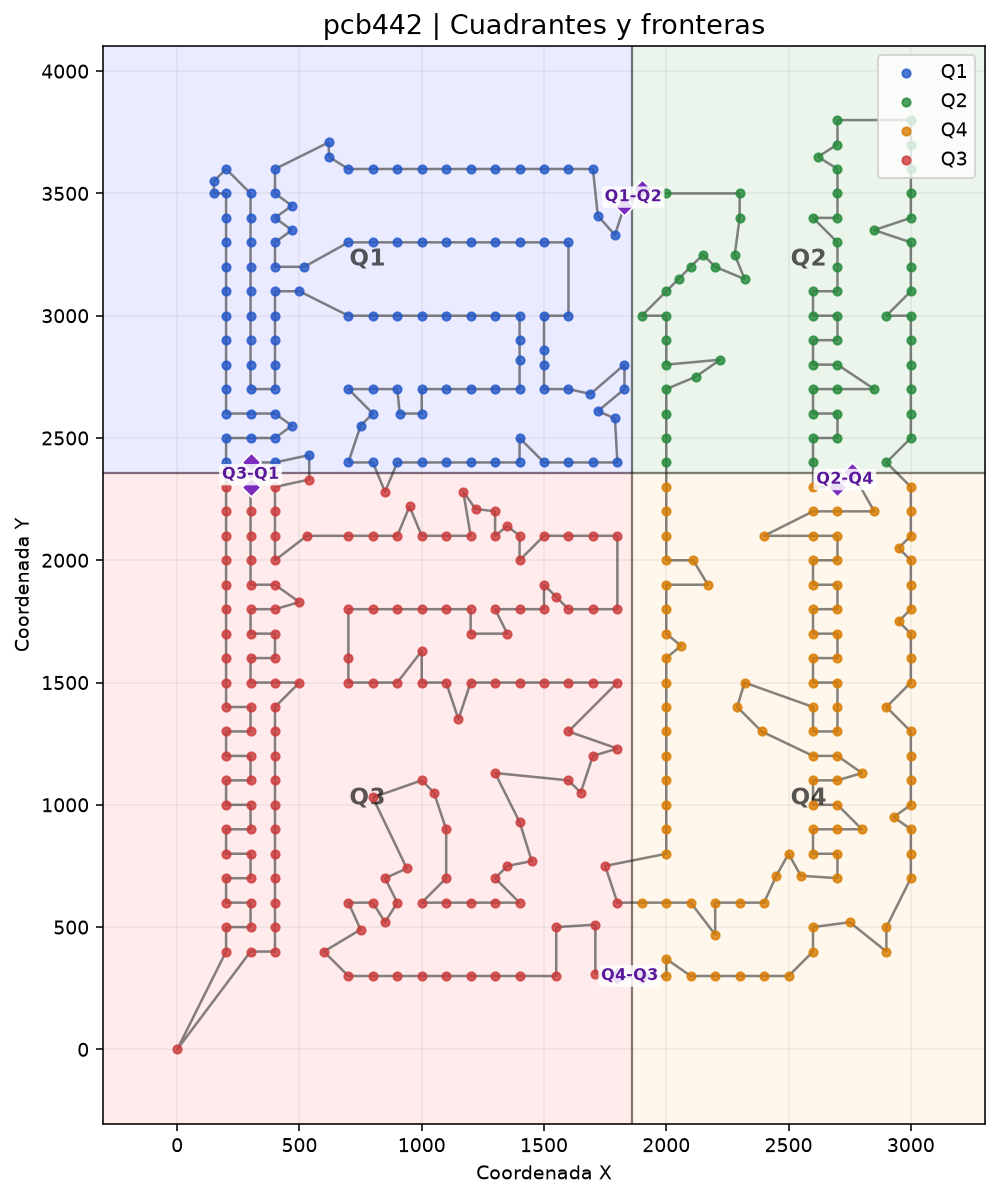
\includegraphics[width=0.70\textwidth]{Resultados_v2/PCB442_QUADRANTS.png}
\caption{Optimal tour on \texttt{pcb442} (50{,}778) colored by quadrant,
with the four selected frontier pairs.}
\label{fig:pcb442-quad}
\end{figure}

\begin{figure}
\centering
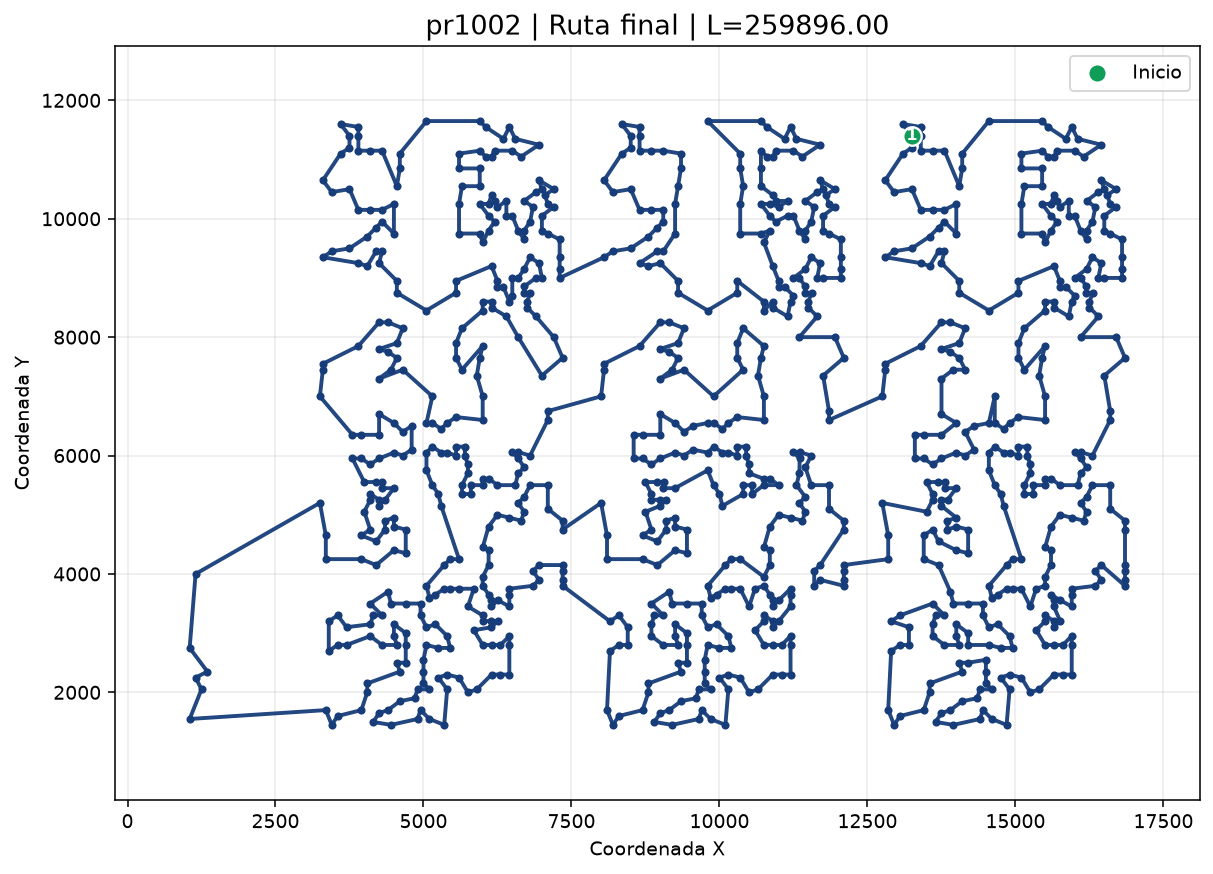
\includegraphics[width=0.70\textwidth]{Resultados_v2/PR1002.png}
\caption{Tour found on \texttt{pr1002} in a single run (259{,}896,
0.329\% above the BKS).}
\label{fig:pr1002-route}
\end{figure}

\subsection{Contribution of the Construction}
\label{sec:ablation}

To isolate the construction, we replace it and keep everything else
fixed: each variant below is followed by exactly the same local search
and ILS, with the same candidate lists, temperature, window, stopping
rule, and seeds.
\begin{itemize}
  \item \textbf{Random + ILS}: a random permutation, a floor with no
    construction information;
  \item \textbf{Nearest Neighbor + ILS}: the classical baseline, started
    at the first city;
  \item \textbf{Partition (no FC) + ILS}: the bounding-box quadrants,
    each routed as a free open path (nearest neighbor plus 2-opt) and
    concatenated in the order $Q_1\!\to\!Q_2\!\to\!Q_4\!\to\!Q_3$, each
    path oriented to join the previous one; no frontier pairs;
  \item \textbf{Frontier Connectivity + ILS}: the same quadrants, with
    the best pair of each frontier as the anchors; a single partition and
    a single frontier combination;
  \item \textbf{GSPH-FC (complete)}: partition portfolio, top-3 pairs per
    frontier, combinations, and funnel.
\end{itemize}

\begin{table}
\caption{Construction ablation on the 63 TSPLIB instances with
$n\le 2{,}000$ (5 runs each, seeds 1000--1004, 315 runs per variant).
Every variant is followed by the same local search and ILS. GAP values
(\%) are averages over instances: of the seed tour, of the first local
optimum (LS), of the best of the five final tours, and of all final
tours. Hits are final tours at the BKS. Times were measured while other
experiments shared the machine and are comparable only within the
table.}
\label{tab:ablation-constr}
\centering\scriptsize
\begin{tabular}{@{}lrrrrrr@{}}
\toprule
\textbf{Construction} & \textbf{GAP seed} & \textbf{GAP LS} & \textbf{GAP best} & \textbf{GAP avg} & \textbf{Hits} & \textbf{Time (s)}\\
\midrule
Random + ILS                 & 1815.62 & 6.17 & 0.037 & 0.117 & 165/315 & 1.31 \\
Nearest Neighbor + ILS       &   24.71 & 4.43 & 0.074 & 0.140 & 168/315 & 1.29 \\
Partition (no FC) + ILS      &   23.50 & 5.44 & 0.040 & 0.101 & 170/315 & 1.27 \\
Frontier Connectivity + ILS  &   13.84 & 6.27 & 0.038 & 0.096 & 172/315 & 1.36 \\
\textbf{GSPH-FC (complete)}  & \textbf{9.95} & \textbf{4.37} & \textbf{0.034} & \textbf{0.080} & \textbf{190/315} & 1.38 \\
\midrule
& \multicolumn{2}{c}{$n\le 300$ (36)} & \multicolumn{2}{c}{$301\le n\le 800$ (12)} & \multicolumn{2}{c}{$801\le n\le 2{,}000$ (15)}\\
\cmidrule(lr){2-3}\cmidrule(lr){4-5}\cmidrule(lr){6-7}
& \textbf{GAP avg} & \textbf{Hits} & \textbf{GAP avg} & \textbf{Hits} & \textbf{GAP avg} & \textbf{Hits}\\
\midrule
Random + ILS                 & 0.030 & 152/180 & 0.106 & 11/60 & 0.333 & 2/75 \\
Nearest Neighbor + ILS       & 0.026 & 161/180 & 0.271 &  7/60 & 0.309 & 0/75 \\
Partition (no FC) + ILS      & 0.046 & 152/180 & 0.083 & 13/60 & \textbf{0.249} & 5/75 \\
Frontier Connectivity + ILS  & 0.021 & 160/180 & 0.079 & 11/60 & 0.289 & 1/75 \\
\textbf{GSPH-FC (complete)}  & \textbf{0.000} & \textbf{174/180} & \textbf{0.078} & \textbf{15/60} & 0.274 & 1/75 \\
\bottomrule
\end{tabular}
\end{table}

Table~\ref{tab:ablation-constr} shows two things. First, the
construction clearly improves the starting point: the complete GSPH-FC
seed is 9.95\% above the BKS, against 24.71\% for nearest neighbor and
23.50\% for the partition without frontier pairs. Choosing frontier
pairs alone lowers the seed GAP to 13.84\%, and the portfolio with
frontier combinations brings it under 10\%. Second, the ILS closes most
of the remaining gap whatever the start: even random tours end at an
average GAP of 0.117\%. Over the 63 instances the complete method ranks
first, with an average GAP of 0.080\% against 0.096--0.140\% and 190 BKS
hits against 165--172, at about the same total time. The differences are
small. A Wilcoxon signed-rank test on per-instance average GAPs finds
the complete method significantly better than the random start
($p=0.029$, 37 non-tied instances), but not than nearest neighbor
($p=0.11$), the partition without frontier pairs ($p=0.46$), or frontier
connectivity with a single combination ($p=0.51$). Two caveats apply to
the breakdown by size. For $n\le 300$ the complete method may polish two
finalists and spends about twice the time of the other variants (0.22~s
against 0.12~s). For $801\le n\le 2{,}000$ the partition without
frontier pairs has the lowest average GAP.

\subsection{Convergence over Time}
\label{sec:convergence}

The ablation leaves a question open: why does a seed that is more than
twice as good (9.95\% against 23.50\% above the BKS) translate into such
a small difference at the end? Either the ILS quickly erases the
differences between starting tours, or the geometric start helps mainly
in the early stages of the search. To tell these apart, we recorded the
best tour found so far over time for three constructions followed by the
same ILS: nearest neighbor, the partition without frontier pairs, and
complete GSPH-FC. We used eight instances from 200 to 1{,}889 cities with
different spatial structure, and 5 runs each. The clock starts after the
distance matrix and candidate lists are built, since this preprocessing
is identical for all variants. Figure~\ref{fig:convergence} shows the
curves and Table~\ref{tab:convergence} summarizes them at fixed fractions
of the run time.

\begin{figure}
\centering
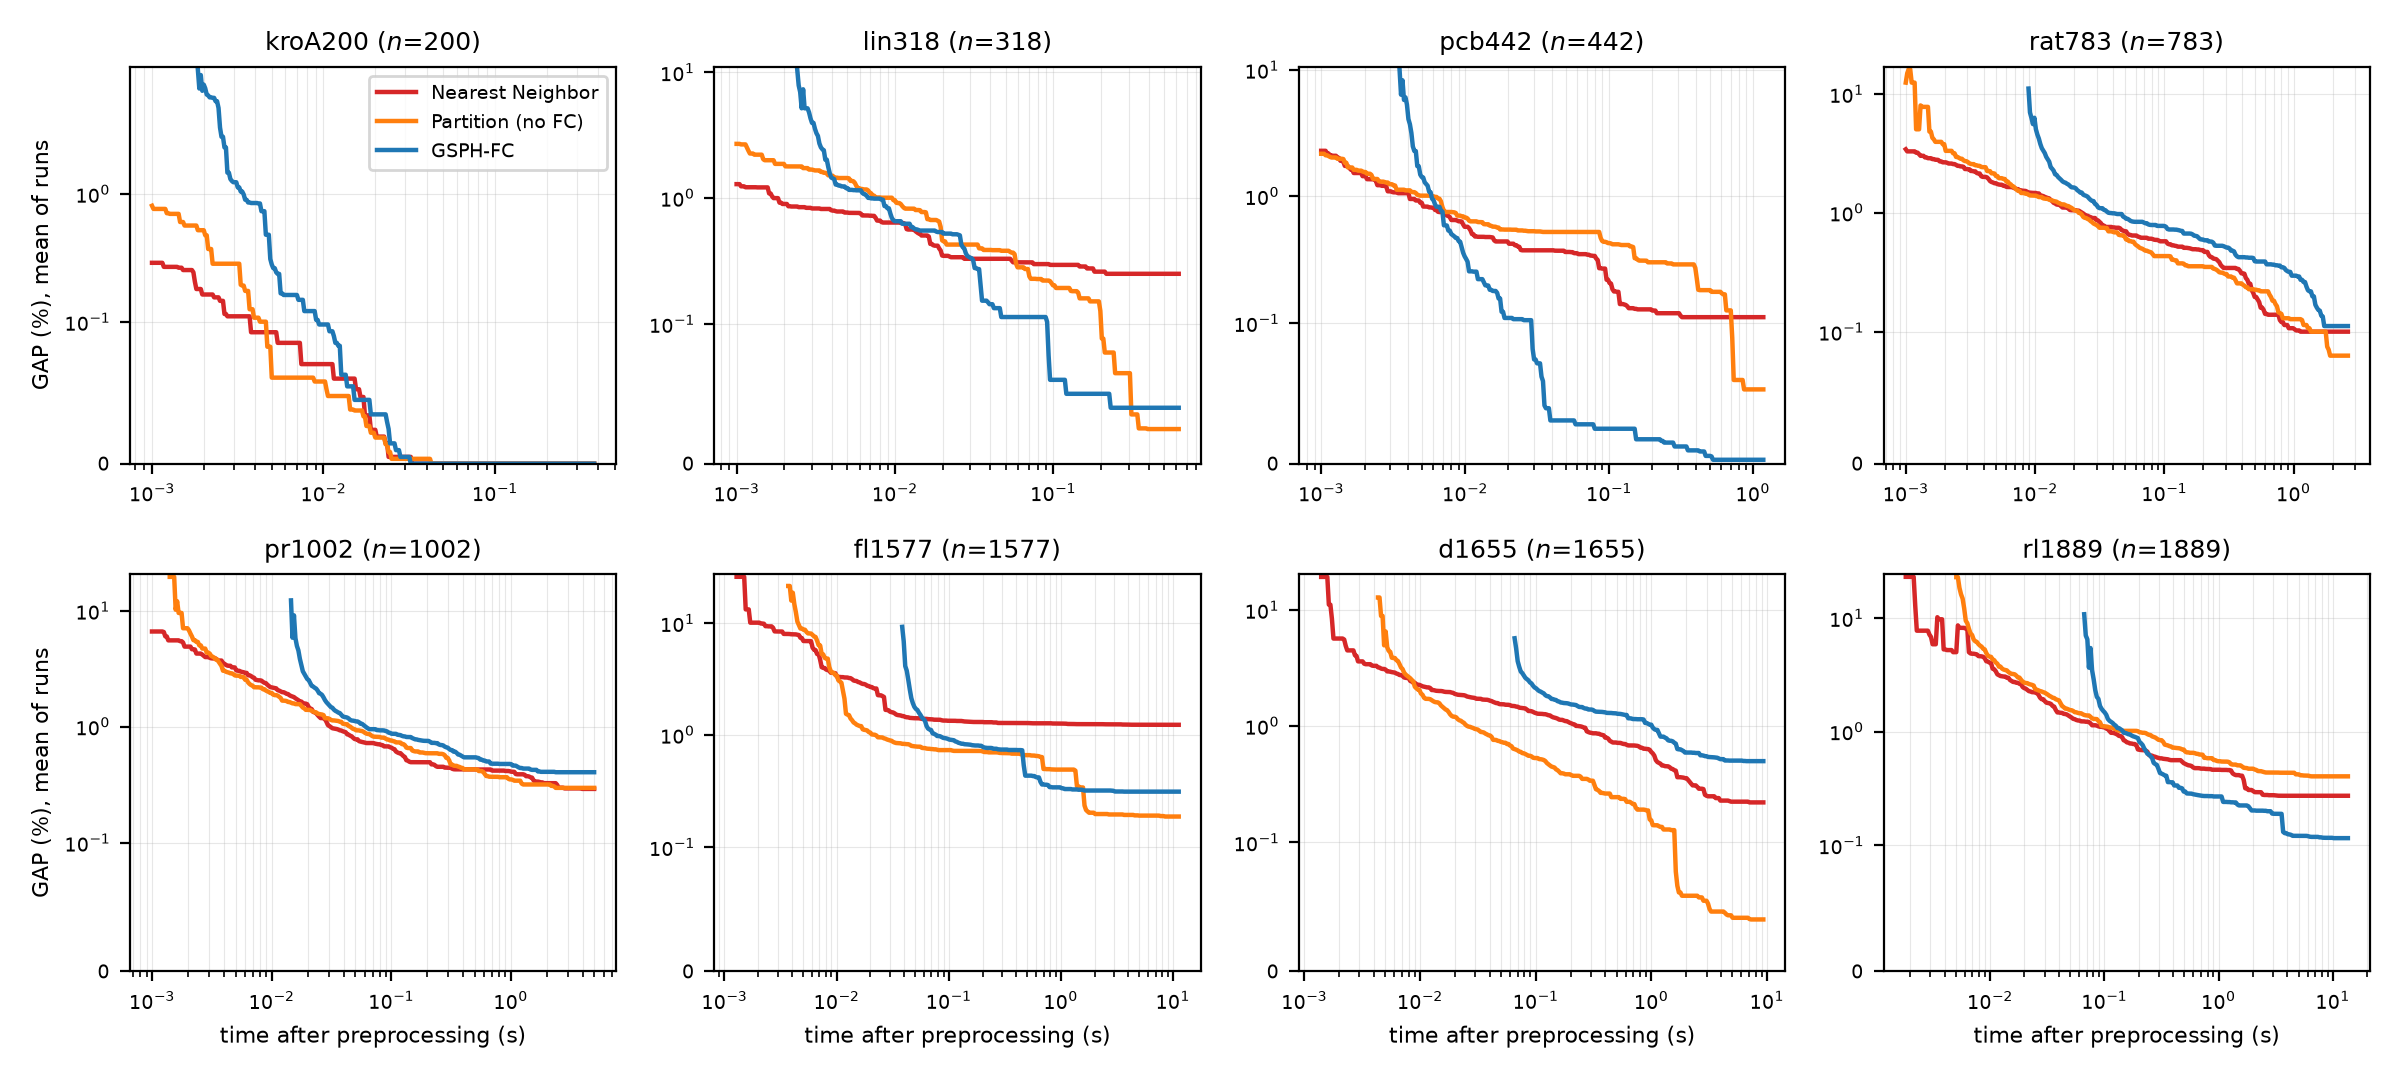
\includegraphics[width=\textwidth]{Resultados_v3/convergencia.png}
\caption{Best GAP found so far versus time after preprocessing (log
scales; mean of 5 runs), for three constructions followed by the same
ILS.}
\label{fig:convergence}
\end{figure}

\begin{table}
\caption{Average GAP (\%) over the eight instances of
Fig.~\ref{fig:convergence} at fixed fractions of the average GSPH-FC
run time on each instance (0.34--9.1~s).}
\label{tab:convergence}
\centering\scriptsize
\begin{tabular}{@{}lrrrrr@{}}
\toprule
\textbf{Construction + ILS} & \textbf{1\%} & \textbf{3\%} & \textbf{10\%} & \textbf{30\%} & \textbf{100\%}\\
\midrule
Nearest Neighbor        & 0.993 & 0.684 & 0.502 & 0.358 & 0.311 \\
Partition (no FC)       & \textbf{0.972} & \textbf{0.604} & \textbf{0.414} & 0.259 & \textbf{0.152} \\
GSPH-FC (complete)      & 2.307 & 0.690 & 0.468 & \textbf{0.255} & 0.186 \\
\bottomrule
\end{tabular}
\end{table}

The second explanation is not supported, and the first one is. The
complete construction has no early lead; it starts behind. It evaluates
several partitions and frontier combinations and brings several seeds
to a local optimum before the ILS begins. As a result, its first
complete tour appears after about 12~ms (median), against 0.5~ms for
nearest neighbor and 1.3~ms for the partition, and at 1\% of the run
time its average GAP is 2.31\% against about 1\% for the other two.
After that the ILS erases most of the differences: by 10\% of the run
time the three variants lie within 0.1 points of each other on average.
The final ranking depends on the instance. The complete construction
ends best on \texttt{pcb442} and \texttt{rl1889} and ties on
\texttt{kroA200} and \texttt{lin318}. It is worse than the partition
without frontier pairs on \texttt{fl1577} (clustered) and \texttt{d1655}
(drilling). Nearest neighbor, in turn, remains at 1.23\% on
\texttt{fl1577}, where both geometric starts end at 0.2--0.3\%. With five
runs per instance these differences are noisy. Together with
Table~\ref{tab:ablation-constr}, however, they indicate that the value
of a geometric start lies less in speed than in avoiding poor regions of
the search space, as nearest neighbor does on clustered instances. They
also show that the full portfolio pays an up-front cost that only pays
off on some instances.

\subsection{Components of the Search Engine}
\label{sec:engine-ablation}

Table~\ref{tab:ablation} isolates the acceptance rule on six instances
chosen for their difficulty (5 runs each, seeds 1000--1004). With $T=0$
the search accepts only non-worsening kicks. On \texttt{kroE100} every
run then ends in the same local optimum (22{,}106, 0.172\%), and three
million additional kicks do not escape it. With $T=0.2\,\bar d$ all five
runs reach the BKS, and the average GAP of \texttt{rat783} drops from
0.509\% to 0.111\%. The perturbation window matters as well: with a
fixed window of 50 positions, \texttt{d1655} stalled at 1.671\% in all
runs, while the size-dependent window $W(n)$ reduced its best GAP to
0.325\% even without the acceptance rule.

\begin{table}
\caption{Effect of the acceptance temperature (5 runs, seeds
1000--1004).}
\label{tab:ablation}
\centering\scriptsize
\begin{tabular}{@{}lrrrrrrr@{}}
\toprule
& & \multicolumn{3}{c}{$T=0$ (non-worsening only)} & \multicolumn{3}{c}{$T=0.2\,\bar d$} \\
\cmidrule(lr){3-5}\cmidrule(lr){6-8}
\textbf{Instance} & $n$ & \textbf{GAP best} & \textbf{GAP avg} & \textbf{Time} & \textbf{GAP best} & \textbf{GAP avg} & \textbf{Time} \\
\midrule
kroE100 &  100 & 0.172 & 0.172 & 0.07 & \textbf{0.000} & 0.000 & 0.09 \\
lin318  &  318 & \textbf{0.000} & 0.054 & 0.28 & \textbf{0.000} & 0.040 & 0.33 \\
pcb442  &  442 & \textbf{0.000} & 0.016 & 0.48 & \textbf{0.000} & 0.003 & 0.59 \\
rat783  &  783 & 0.261 & 0.509 & 1.15 & 0.023 & 0.111 & 1.90 \\
pr1002  & 1002 & 0.294 & 0.459 & 1.94 & 0.326 & 0.404 & 2.22 \\
d1655   & 1655 & 0.325 & 0.653 & 4.50 & 0.034 & 0.499 & 5.26 \\
\midrule
\textit{Average} & & 0.175 & 0.311 & 1.40 & 0.064 & 0.176 & 1.73 \\
\bottomrule
\end{tabular}
\end{table}

The engine design also explains the running times. An earlier
implementation with the same construction, but with an uncompiled
search, full-tour copies on rejection, and a fixed time budget of
5--30~s per run, performed about 290 ILS iterations per second on
\texttt{pcb442}; the localized engine performs about 420 thousand. On
the 37 instances that the earlier implementation was run on, it reached
the BKS on 22 with 14.65~s per run on average, while GSPH-FC reaches it
on all 37 with 0.23~s per run, about 65 times faster. Both were measured
on the same machine.

\subsection{Parameter Sensitivity}
\label{sec:sensitivity}

Table~\ref{tab:sensitivity} varies one parameter at a time around its
default value. To avoid tuning on a narrow sample, we use 16 instances
from 100 to 1{,}889 cities with different spatial distributions: uniform
random (\texttt{kroA100}, \texttt{ch150}, \texttt{kroB200},
\texttt{rd400}), clustered (\texttt{fl417}, \texttt{fl1400}), drilling
and printed-circuit layouts (\texttt{a280}, \texttt{pcb442},
\texttt{d493}, \texttt{rat783}, \texttt{u1060}, \texttt{pcb1173},
\texttt{d1655}), and three further TSPLIB instances (\texttt{pr1002},
\texttt{vm1748}, \texttt{rl1889}). Each variant is run 5 times (seeds
1000--1004) on each instance.

\begin{table}
\caption{One-at-a-time parameter sensitivity on 16 instances (5 runs
each, 80 runs per variant). GAP avg (\%) is averaged over all instances
and over the eight with $n\le 500$ and the eight with $n>500$. Hits are
runs at the BKS. Times were measured while other experiments shared the
machine and are comparable only within the table.}
\label{tab:sensitivity}
\centering\scriptsize
\begin{tabular}{@{}llrrrrr@{}}
\toprule
& & \multicolumn{3}{c}{\textbf{GAP avg}} & & \\
\cmidrule(lr){3-5}
\textbf{Parameter} & \textbf{Value} & \textbf{All} & $n\le 500$ & $n>500$ & \textbf{Hits} & \textbf{Time (s)}\\
\midrule
\multicolumn{2}{@{}l}{\textit{Default} ($k{=}3$, portfolio, $T{=}0.2\bar d$, $n/8$, $300n$)} & 0.149 & 0.027 & 0.270 & 29/80 & 2.56 \\
\midrule
Pairs per frontier $k$     & 1 & 0.152 & 0.042 & 0.263 & 29/80 & 2.64 \\
                           & 5 & 0.169 & 0.068 & 0.270 & 27/80 & 2.55 \\
Partition portfolio        & bbox only & 0.177 & 0.089 & 0.264 & 22/80 & 2.39 \\
Temperature $T/\bar d$     & 0   & 0.257 & 0.068 & 0.445 & 29/80 & 2.02 \\
                           & 0.1 & 0.177 & 0.039 & 0.315 & 24/80 & 2.40 \\
                           & 0.4 & 0.164 & 0.047 & 0.280 & 19/80 & 2.04 \\
Window divisor ($n/\cdot$) & 4  & 0.152 & 0.023 & 0.281 & 28/80 & 3.18 \\
                           & 16 & 0.241 & 0.024 & 0.458 & 24/80 & 2.20 \\
Stall factor ($\cdot\,n$)  & 100  & 0.209 & 0.039 & 0.379 & 19/80 & 0.93 \\
                           & 1000 & 0.110 & 0.020 & 0.201 & 33/80 & 7.27 \\
\bottomrule
\end{tabular}
\end{table}

Most differences appear on the larger instances. For $n\le 500$
nearly every variant ends within a few hundredths of a percent of the
BKS, so the choice of parameters matters mainly for $n>500$. Four
conclusions follow.

\emph{Acceptance and window.} These are the parameters that most need
to be right. Without the acceptance rule ($T=0$) the average GAP for
$n>500$ rises from 0.270\% to 0.445\%, and the default is better on 10
of the 16 instances and worse on only 2. Values of $T/\bar d$ between
0.1 and 0.4 are all reasonable, and 0.2 has the lowest average. A
window of $n/16$ is clearly too small (0.458\% for $n>500$, and 0.41\%
against 0.10\% on the clustered instances). A window of $n/4$ matches
the default in quality but takes about 24\% more time, so $n/8$ is the
better compromise.

\emph{Frontier pairs.} The number of pairs per frontier hardly matters.
With five pairs, the average result is identical to the default on 15
of the 16 instances, because only the best-ranked three to five
combinations are assembled. With a single pair, the result is worse on
6 instances and better on 3.

\emph{Partition portfolio.} Its effect depends on the spatial structure
of the instance. With the bounding-box partition alone, the clustered
instances improve markedly (0.007\% against 0.104\%), while the drilling
and other instances get worse, and the variant reaches the BKS less
often (22 against 29 runs). This matches the convergence curves, where
the single partition without frontier pairs was also better on
\texttt{fl1577}. The portfolio is therefore a reasonable default, not a
universal improvement.

\emph{Stall factor.} This is a pure time--quality knob, not a tuning
parameter. A factor of $1000n$ improves the average GAP from 0.149\% to
0.110\% and is better than the default on 10 instances and worse on
none, but it takes 2.8 times longer. A factor of $100n$ is about 2.7
times faster at 0.209\%. The default $300n$ is a middle point. A user with a
larger time budget should raise this factor rather than change any
other parameter.

\subsection{Comparison with LKH}
\label{sec:lkh}

LKH~\cite{helsgaun2000effective,helsgaun2017extension} is the reference
heuristic for the symmetric TSP. We ran LKH-3 (version 3.0.8, through
the \texttt{elkai} Python binding, which embeds the original C code) on
the same instances and seeds in two settings: with its default
parameters (one run of $n$ trials per seed), and with a time limit equal
to the average GSPH-FC time per run on that instance. LKH does not count
its preprocessing (subgradient ascent for the $\alpha$-nearness
candidates) towards that limit, so we report the total wall-clock time.
Every LKH tour was validated and its length recomputed under
\texttt{EUC\_2D}.

\begin{table}
\caption{GSPH-FC versus LKH-3 on the 63 TSPLIB instances with
$n\le 2{,}000$. GSPH-FC: 10 runs per instance. LKH: 3 runs per instance
(seeds 1000--1002), with default parameters and with a time limit equal
to the average GSPH-FC time. GAP avg (\%) and time (s) are averages over
instances; hits are runs at the BKS.}
\label{tab:lkh}
\centering\scriptsize
\begin{tabular}{@{}lrrrrrrrrr@{}}
\toprule
& \multicolumn{3}{c}{\textbf{GSPH-FC}} & \multicolumn{3}{c}{\textbf{LKH default}} & \multicolumn{3}{c}{\textbf{LKH, same time}}\\
\cmidrule(lr){2-4}\cmidrule(lr){5-7}\cmidrule(lr){8-10}
\textbf{Range} & \textbf{GAP} & \textbf{Hits} & \textbf{Time} & \textbf{GAP} & \textbf{Hits} & \textbf{Time} & \textbf{GAP} & \textbf{Hits} & \textbf{Time}\\
\midrule
$n\le 300$ (36)           & 0.001 & 342/360 & 0.22 & 0.001 & 105/108 &  0.12 & 0.001 & 105/108 & 0.10 \\
$301\le n\le 800$ (12)    & 0.081 &  25/120 & 0.82 & 0.010 &  31/36  &  2.06 & 0.010 &  30/36  & 0.88 \\
$801\le n\le 2{,}000$ (15)& 0.301 &   1/150 & 3.63 & 0.041 &  21/45  & 14.55 & 0.073 &  16/45  & 4.52 \\
\midrule
\textit{All} (63)         & 0.088 & 368/630 & 1.14 & 0.012 & 157/189 &  3.93 & 0.020 & 151/189 & 1.30 \\
\bottomrule
\end{tabular}
\end{table}

LKH is the stronger heuristic (Table~\ref{tab:lkh}), as expected from a
mature solver built on $\alpha$-nearness candidates and 5-opt sequential
moves. For $n\le 300$ both methods reach the BKS in almost every run,
and LKH needs about half the time. In the intermediate range LKH reaches
an average GAP of 0.010\% against 0.081\% for GSPH-FC, both with its
default settings (2.5 times slower than GSPH-FC) and when limited to the
GSPH-FC time. For $801\le n\le 2{,}000$ the difference grows: 0.041\%
for LKH with its default settings, which take four times longer,
0.073\% at the same time, and 0.301\% for GSPH-FC. Over the 63
instances, GSPH-FC has a lower average GAP than LKH on only three
(\texttt{ch150}, \texttt{lin318}, and \texttt{fl1577} at equal time),
ties on 29, and is worse on the rest.

% ================================================================
\section{Discussion}
\label{sec:discussion}
% ================================================================

\paragraph{What each phase contributes.} The ablation and the
convergence curves give a consistent picture. The frontier-conditioned
construction produces the best seeds and, at the end, the most BKS hits
and the lowest average GAP over 63 instances. The localized ILS,
however, accounts for most of the final quality, and it erases the
differences between seeds quickly: even random tours end within 0.12\%
of the BKS on average. The benefit of a geometric start is mainly one of
robustness. Starting from the quadrant structure avoids poor basins,
such as the 1.23\% at which nearest neighbor stalls on \texttt{fl1577},
rather than giving an early lead. The full portfolio, which builds and
polishes several seeds, has an up-front cost of about 10~ms and pays off
on some instances (\texttt{pcb442}, \texttt{rl1889}) but not on others
(\texttt{fl1577}, \texttt{d1655}). This suggests a lighter variant, with
a single partition and frontier pairs, for settings where a usable tour
is needed within milliseconds. Because iterations cost microseconds, the
engine reaches the BKS on all instances up to 300 cities in well under a
second. We regard the honest separation of the two contributions as
part of the result: the geometric idea is sound and interpretable, but
it should not be credited with quality that the search engine delivers.

\paragraph{Positioning.} GSPH-FC does not compete with LKH on solution
quality beyond a few hundred cities, and we do not claim otherwise. Its
case rests on other grounds: a construction that can be read and drawn,
a short Python code base with compiled kernels, results within a few
tenths of a percent of the optimum in seconds, and a single parameter,
$S(n)$, that moves the method along its time--quality curve
(Section~\ref{sec:sensitivity}).

\paragraph{Limitations.} First, beyond roughly 10{,}000 cities the
array representation makes each reversal $O(n)$, runs end at the 60~s
cap before stagnation, and the dense distance matrix becomes the memory
bottleneck. Second, strongly clustered instances such as
\texttt{fl3795} show a large spread between runs, which suggests that
kicks crossing clusters are under-represented. Third, axis-aligned
quadrants may be a poor fit for elongated or diagonally clustered
instances. Fourth, the ablation and the LKH comparison cover instances
up to 2{,}000 cities with 3--5 runs each; larger studies would sharpen
the small differences between constructions. Natural next steps are a
variable-depth move (Or-3opt or Lin--Kernighan style) inside the same
reversal framework, two-level doubly-linked lists with distances
computed on the fly for the largest instances, adaptive partition
orientations, and asymmetric costs from real road networks.

% ================================================================
\section{Conclusions}
\label{sec:conclusions}
% ================================================================

GSPH-FC combines a geometric construction in which the connections
between quadrants are decided before the quadrants are routed with a
localized ILS whose iterations cost microseconds. On 77 TSPLIB instances
it reaches the BKS on 44, including all instances with $n\le 300$ in
under half a second, and stays within 0.60\% of the BKS up to 6{,}000
cities. Measuring the two phases separately shows that frontier
connectivity yields the best starting tours and the most consistent
results, while the localized ILS accounts for most of the final quality.
Convergence curves show that this advantage is not an early one: the
ILS erases most of the differences between seeds within the first tenth
of the run, and a geometric start helps mainly by avoiding poor basins
on clustered instances.
GSPH-FC matches LKH-3 on small instances but not beyond 300 cities,
which positions it as a lightweight and interpretable alternative rather
than a replacement. All tables and figures can be reproduced with the
accompanying scripts.

% BLIND REVIEW: acknowledgements hidden
%
% RESTORE BEFORE FINAL SUBMISSION:
%\begin{credits}
%\subsubsection{\ackname}
%The authors thank the faculty of the Heuristics course at
%Universidad Andres Bello for their guidance and material support
%during the development of this work.
%\end{credits}

\bibliographystyle{splncs04}
\bibliography{bibliografia}

\end{document}
